\documentclass{beamer}
\usepackage[polish,british]{babel}
\usepackage[utf8]{inputenc}
\usepackage{enumerate}
\usepackage{tabu}
\setbeamertemplate{itemize item}[square]
\setbeamertemplate{itemize subitem}[circle]

\author{Paweł Paczuski \\ \texttt{p.paczuski@stud.elka.pw.edu.pl}}
\title{Structured reporting system}
\date{06.04.2018}
\begin{document}
\begin{frame}
\titlepage
\end{frame}

\section*{Outline}
\begin{frame}
\frametitle{Outline}
\tableofcontents
\end{frame}

\section{Introduction}
\subsection{Problems of modern medicine}
\begin{frame}
\frametitle{Areas of interest of modern medicine}
\begin{itemize}
	\item increasing variety of diagnostic techniques and procedures
	\item unsatisfiable demand for medical services
	\item bureaucracy
	\item huge volumes of data to process and store. \alert{Healthcare Informatics}
\end{itemize}
\end{frame}

\begin{frame}
\frametitle{Healthcare Informatics vs Computer Science}
\begin{tabu}{XX}
	\rowfont{\bfseries\itshape\large} Computer Science & Healthcare Informatics\\
	\hline
	general field & information engineering applied to the health care \\ \hline
	data structures, algorithms & flow of information\\ \hline
	ways of persistently storing data        & ways of presenting data at proper time to proper person\\ \hline
\end{tabu}
\end{frame}

\subsection{Standards}
\begin{frame}
\frametitle{Healthcare standards}
\begin{itemize}
	\item medical nomenclature SNOMED CT, LOINC
	\item exchange protocols and formats HL7, DICOM
\end{itemize}
\begin{figure}
	\centering
	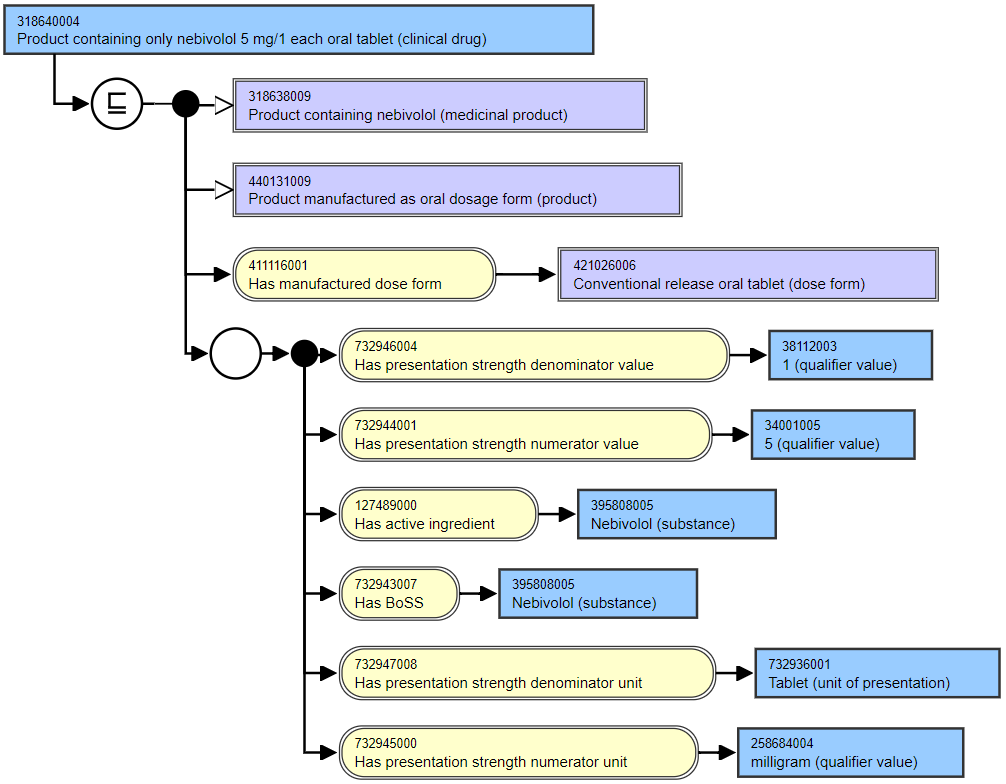
\includegraphics[width=0.7\linewidth]{../snomed}
	\caption{Drug product example in SNOMED CT}
	\label{fig:snomed}
\end{figure}

\end{frame}

\subsection{Typical workflow of a radiologist}
\begin{frame}
\frametitle{Typical workflow of a radiologist}
\begin{figure}
	\centering
	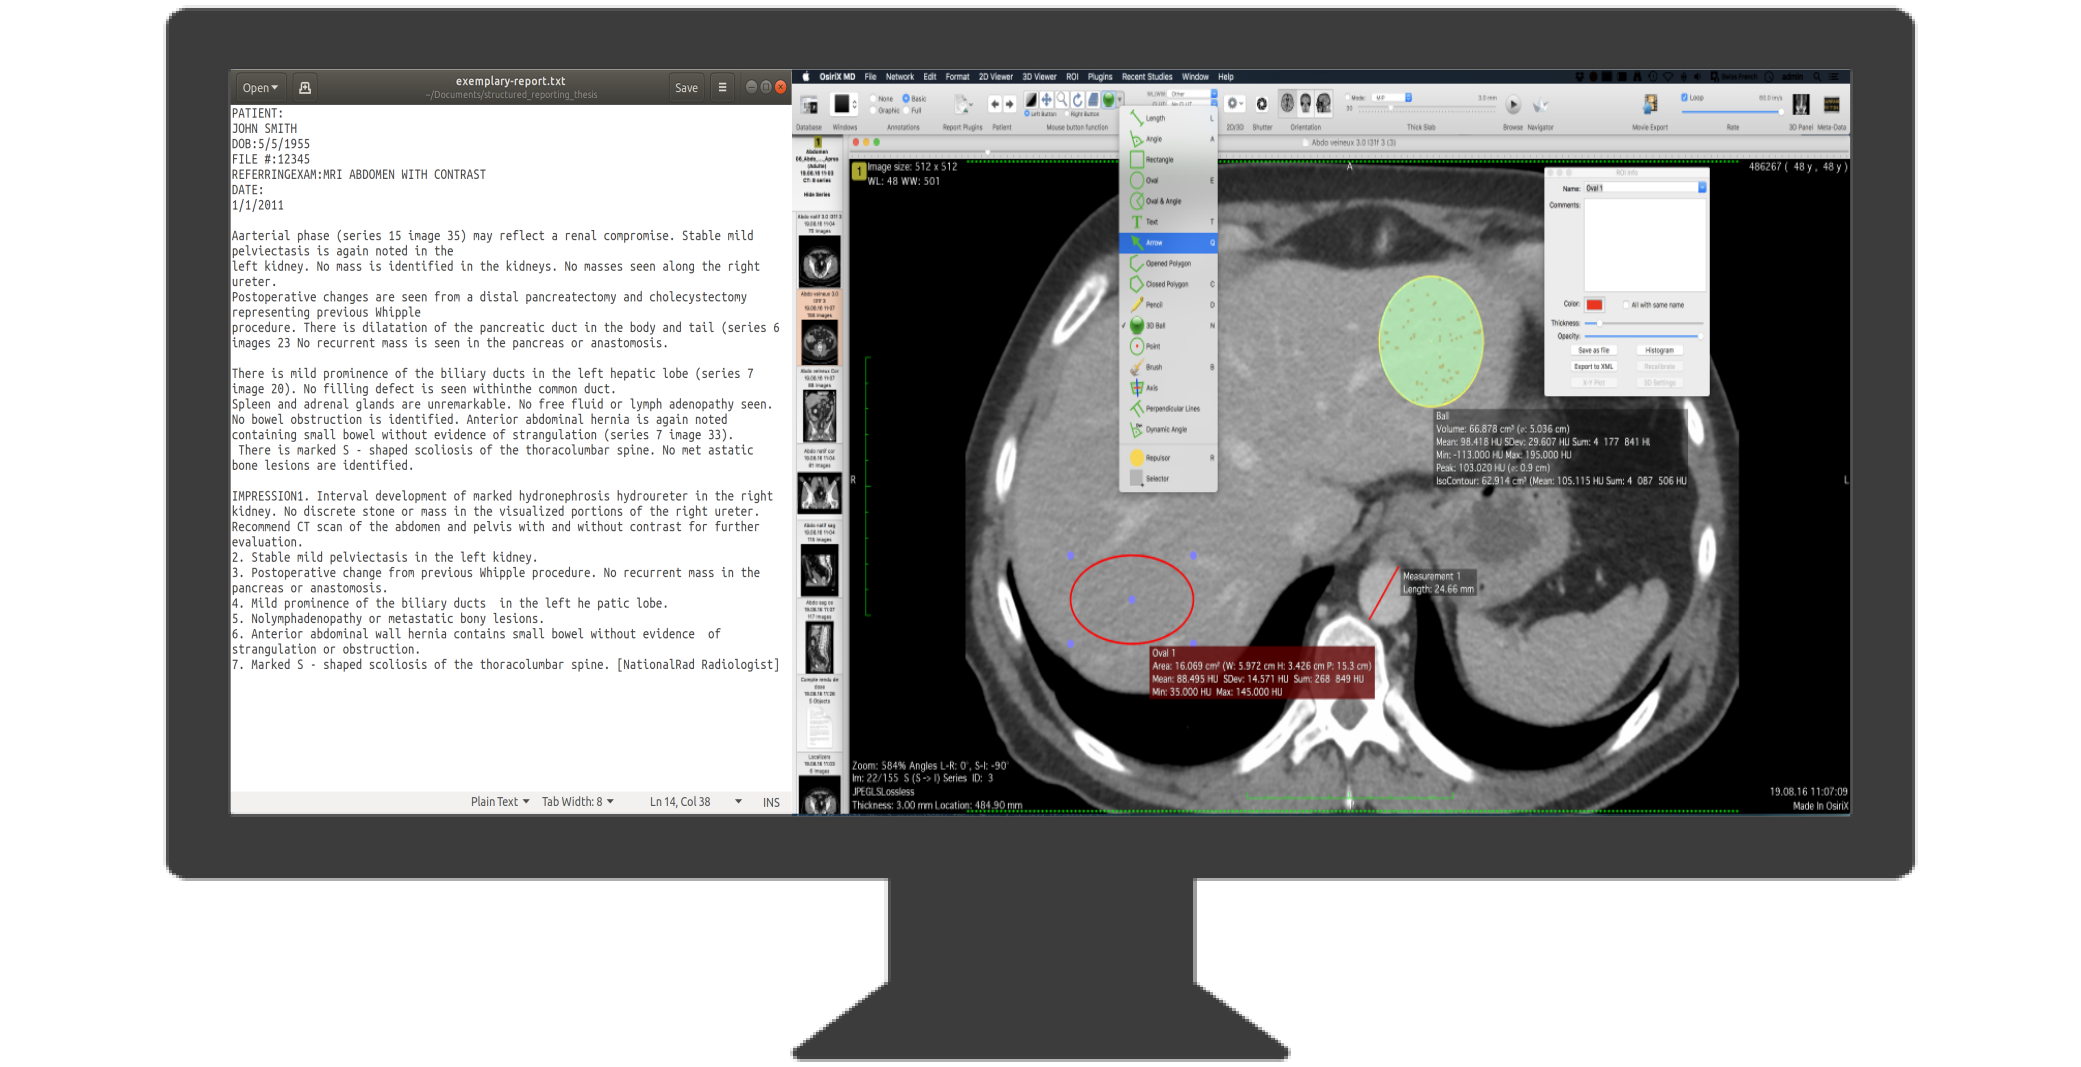
\includegraphics[width=1\linewidth]{../workspace}
	\caption{Typically, a radiologist analyzes medical images and creates report's text simultaneously}
	\label{fig:workspace}
\end{figure}
\end{frame}

\begin{frame}
\frametitle{Areas of optimization}
What can be improved:
\begin{itemize}
	\item radiologists are \alert{very BAD} at typing on keyboard
	\item speech recognition has problems with capturing medical language
	\item reporting quality  
\end{itemize}

How:
\begin{itemize}
	\item typing on keyboard replaced by checking boxes with predefined phrases
	\item reports represented as trees that have relations between causes and effects
	\item workflow organized around set of checklists and \alert{templates}
\end{itemize}
\end{frame}


\section{Design and implementation of Structured reporting system}
\subsection{Radiological report as a tree}

\begin{frame}
\frametitle{Modified workflow}
\begin{figure}
	\centering
	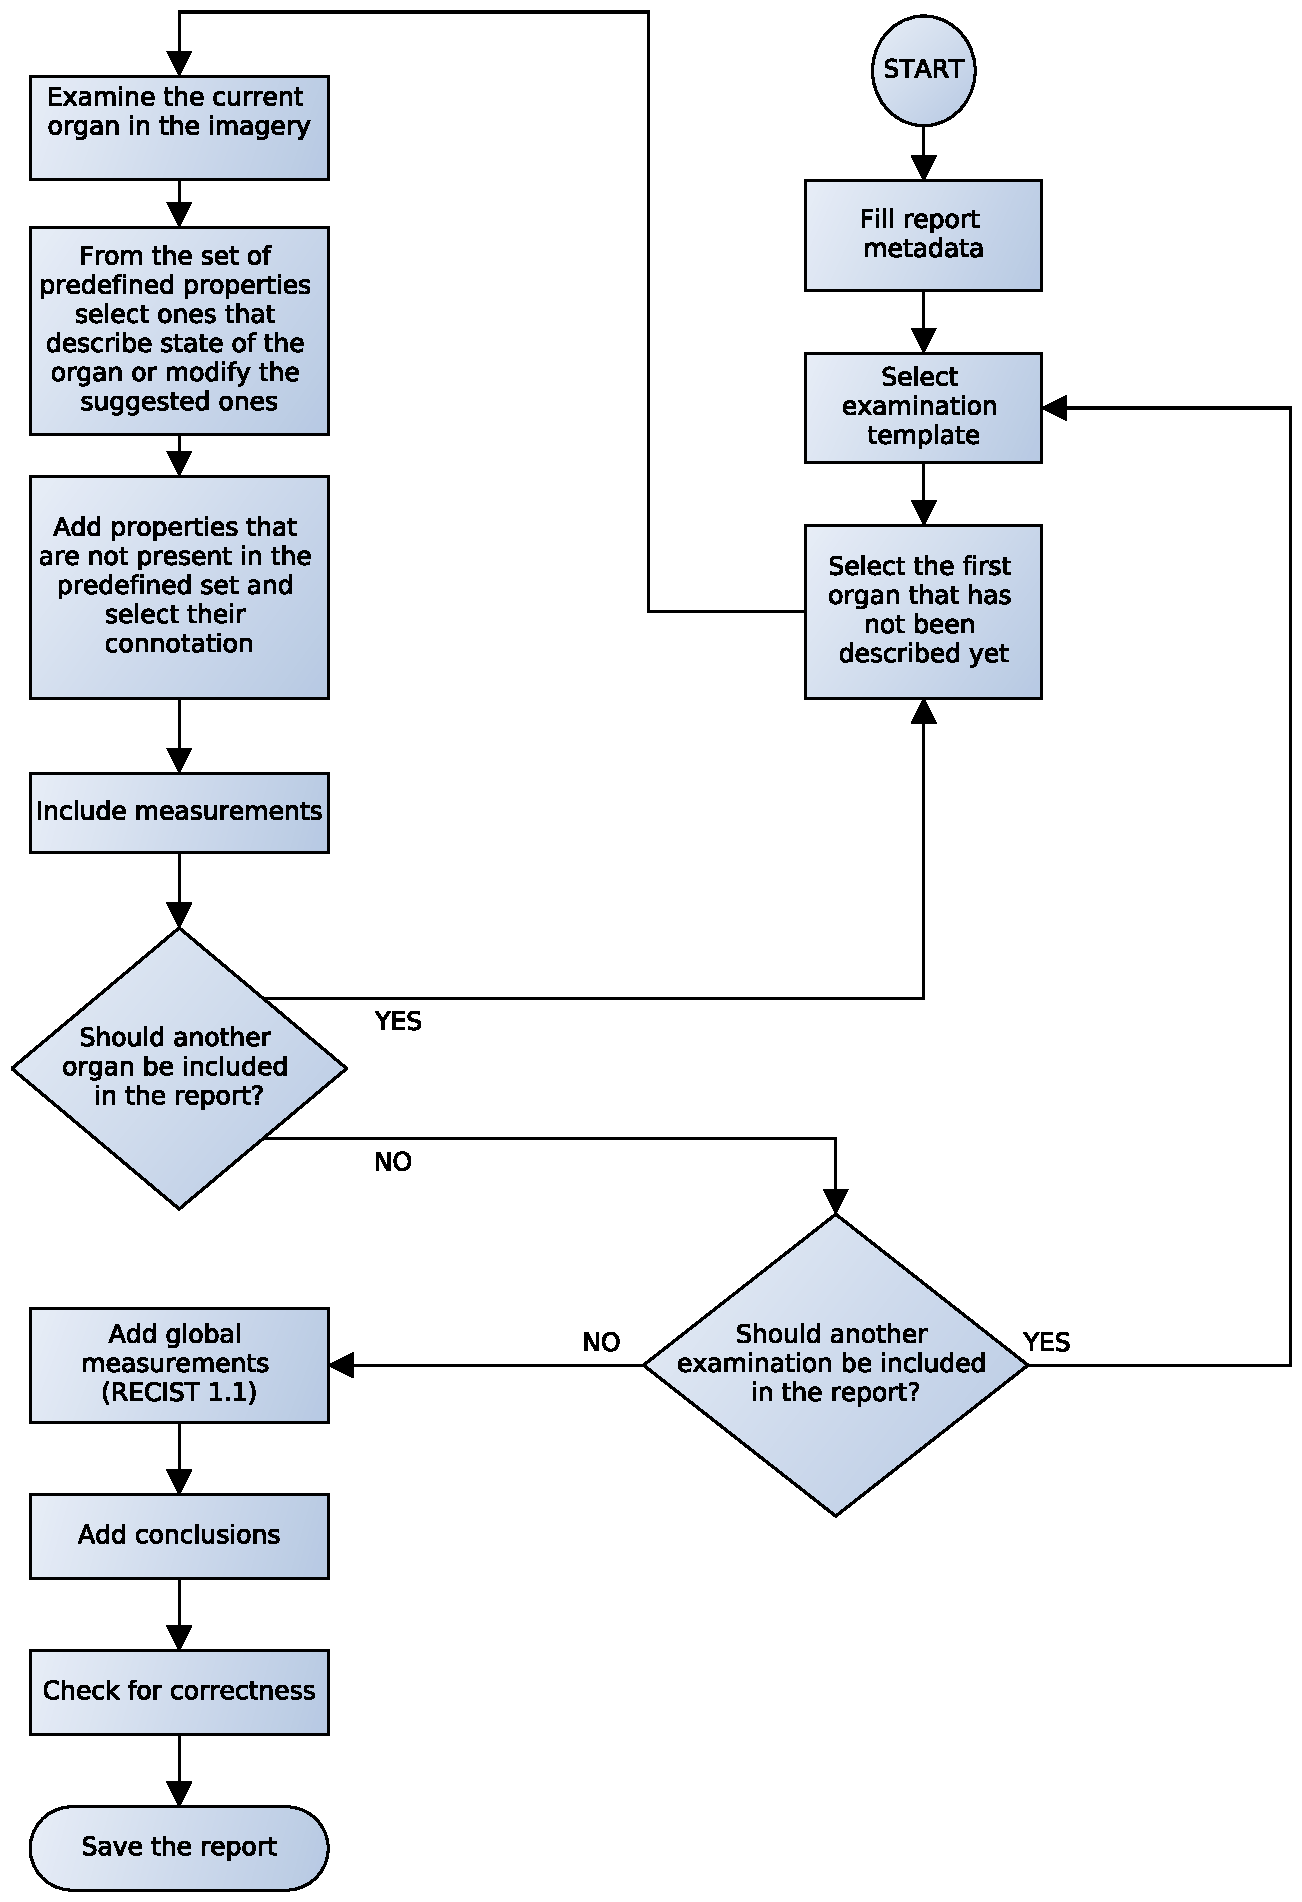
\includegraphics[width=0.5\linewidth]{../report-workflow}
	\label{fig:report-workflow}
\end{figure}
\end{frame}


\begin{frame}
\frametitle{Reporting ontology}
\begin{figure}
	\centering
	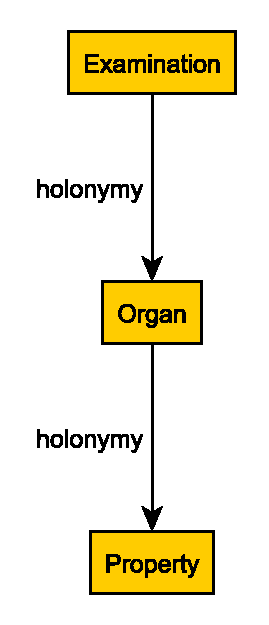
\includegraphics[width=0.2\linewidth]{../report-semantic}
	\caption{Types of entities and relations between them}
	\label{fig:report-ontology}
\end{figure}
\end{frame}


\begin{frame}
\frametitle{Radiological report as a tree}
\begin{figure}
\centering
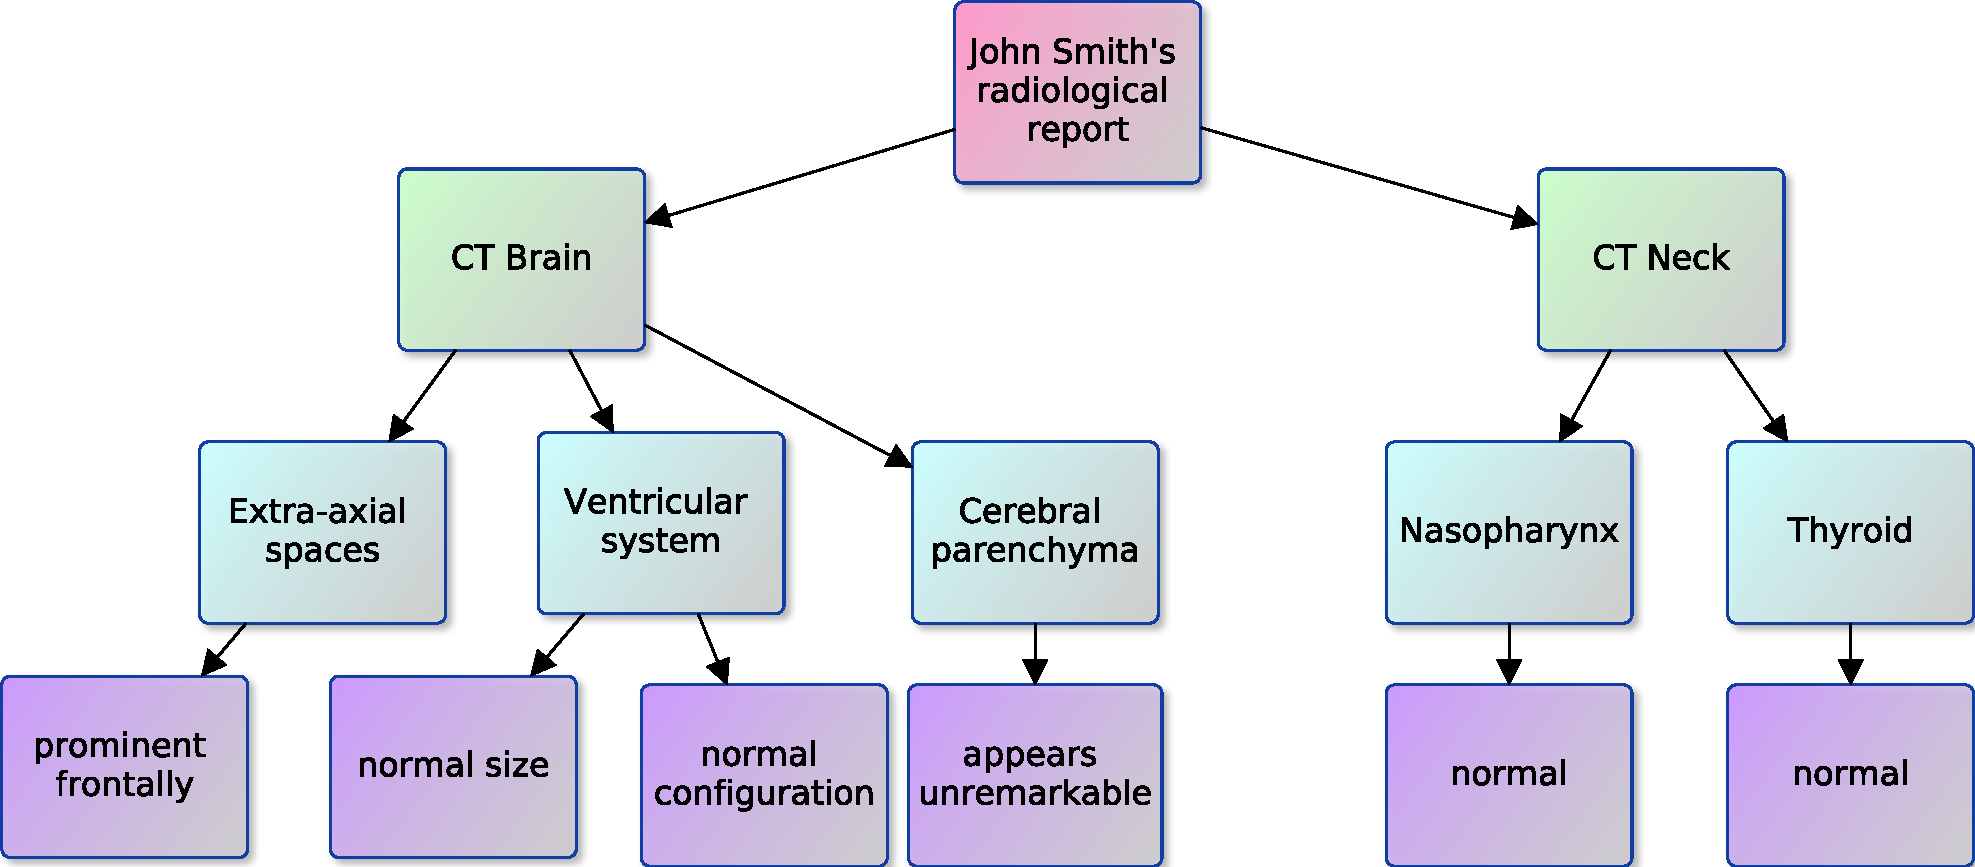
\includegraphics[width=1\linewidth]{../report-tree}
\label{fig:report-tree}
\end{figure}
\end{frame}

\begin{frame}
\frametitle{Textual representation}
\begin{figure}
\centering
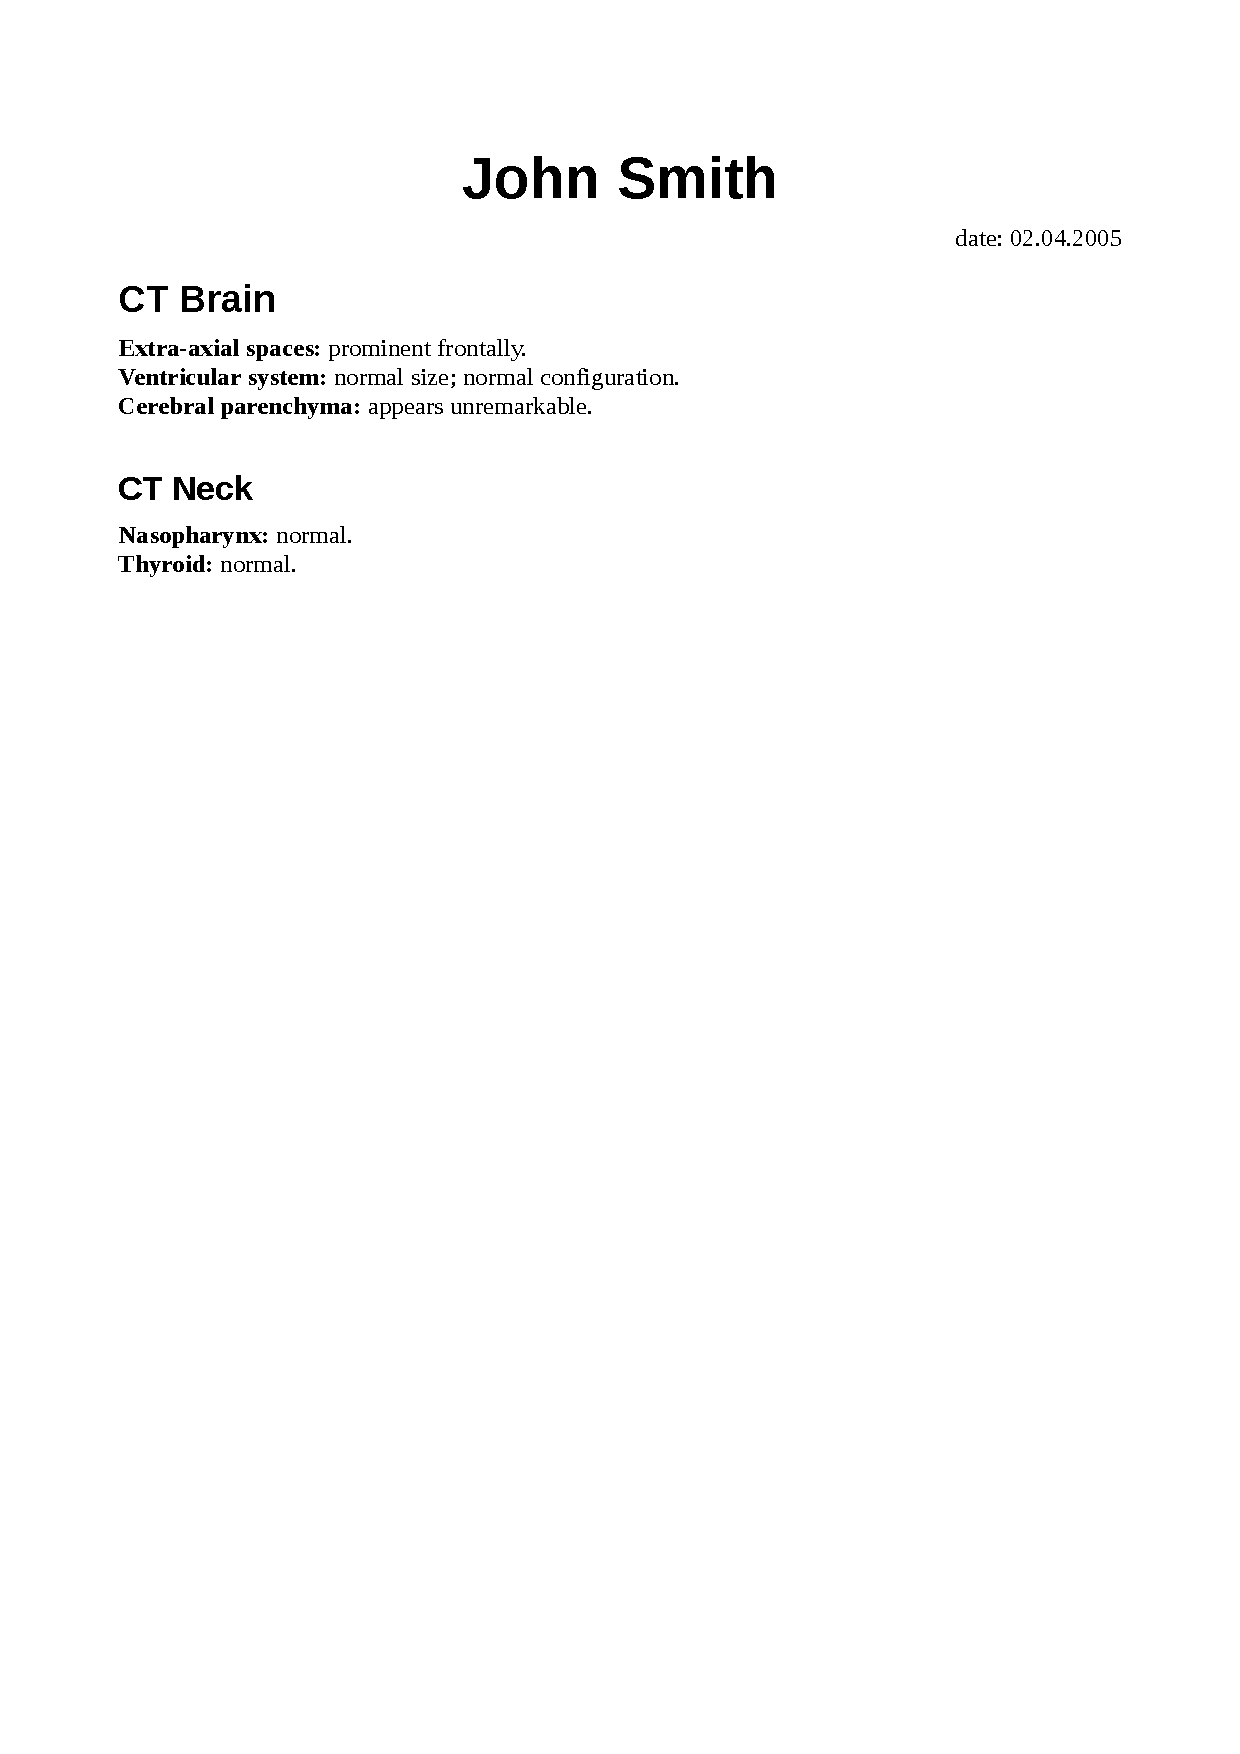
\includegraphics[width=\linewidth]{../rendered-report}
\label{fig:rendered-report}
\end{figure}
\end{frame}

\subsection{Technological stack}
\begin{frame}
\frametitle{Technological stack}
\begin{itemize}
	\item backend 
	\begin{itemize}
		\item C\#
		\item ASP.NET
		\item MS SQL 
	\end{itemize}
	\item frontend (hybrid approach)
	\begin{itemize}
		\item AngularJS, ES5 
	\end{itemize}
\end{itemize}

\end{frame}

\subsection{User interface}
\begin{frame}
\frametitle{Report metadata}
\begin{figure}
	\centering
	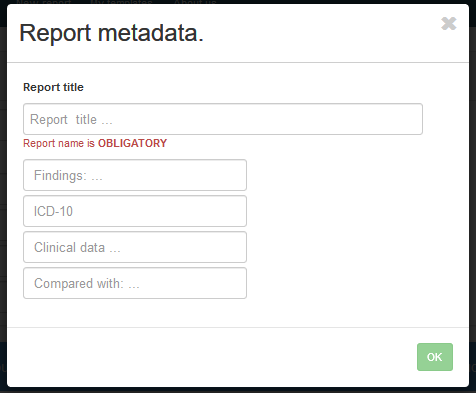
\includegraphics[width=0.6\linewidth]{../report-metadata}
	\label{fig:report-metadata}
\end{figure}
\end{frame}

\begin{frame}
\frametitle{Report editor interface}
\begin{figure}
	\centering
	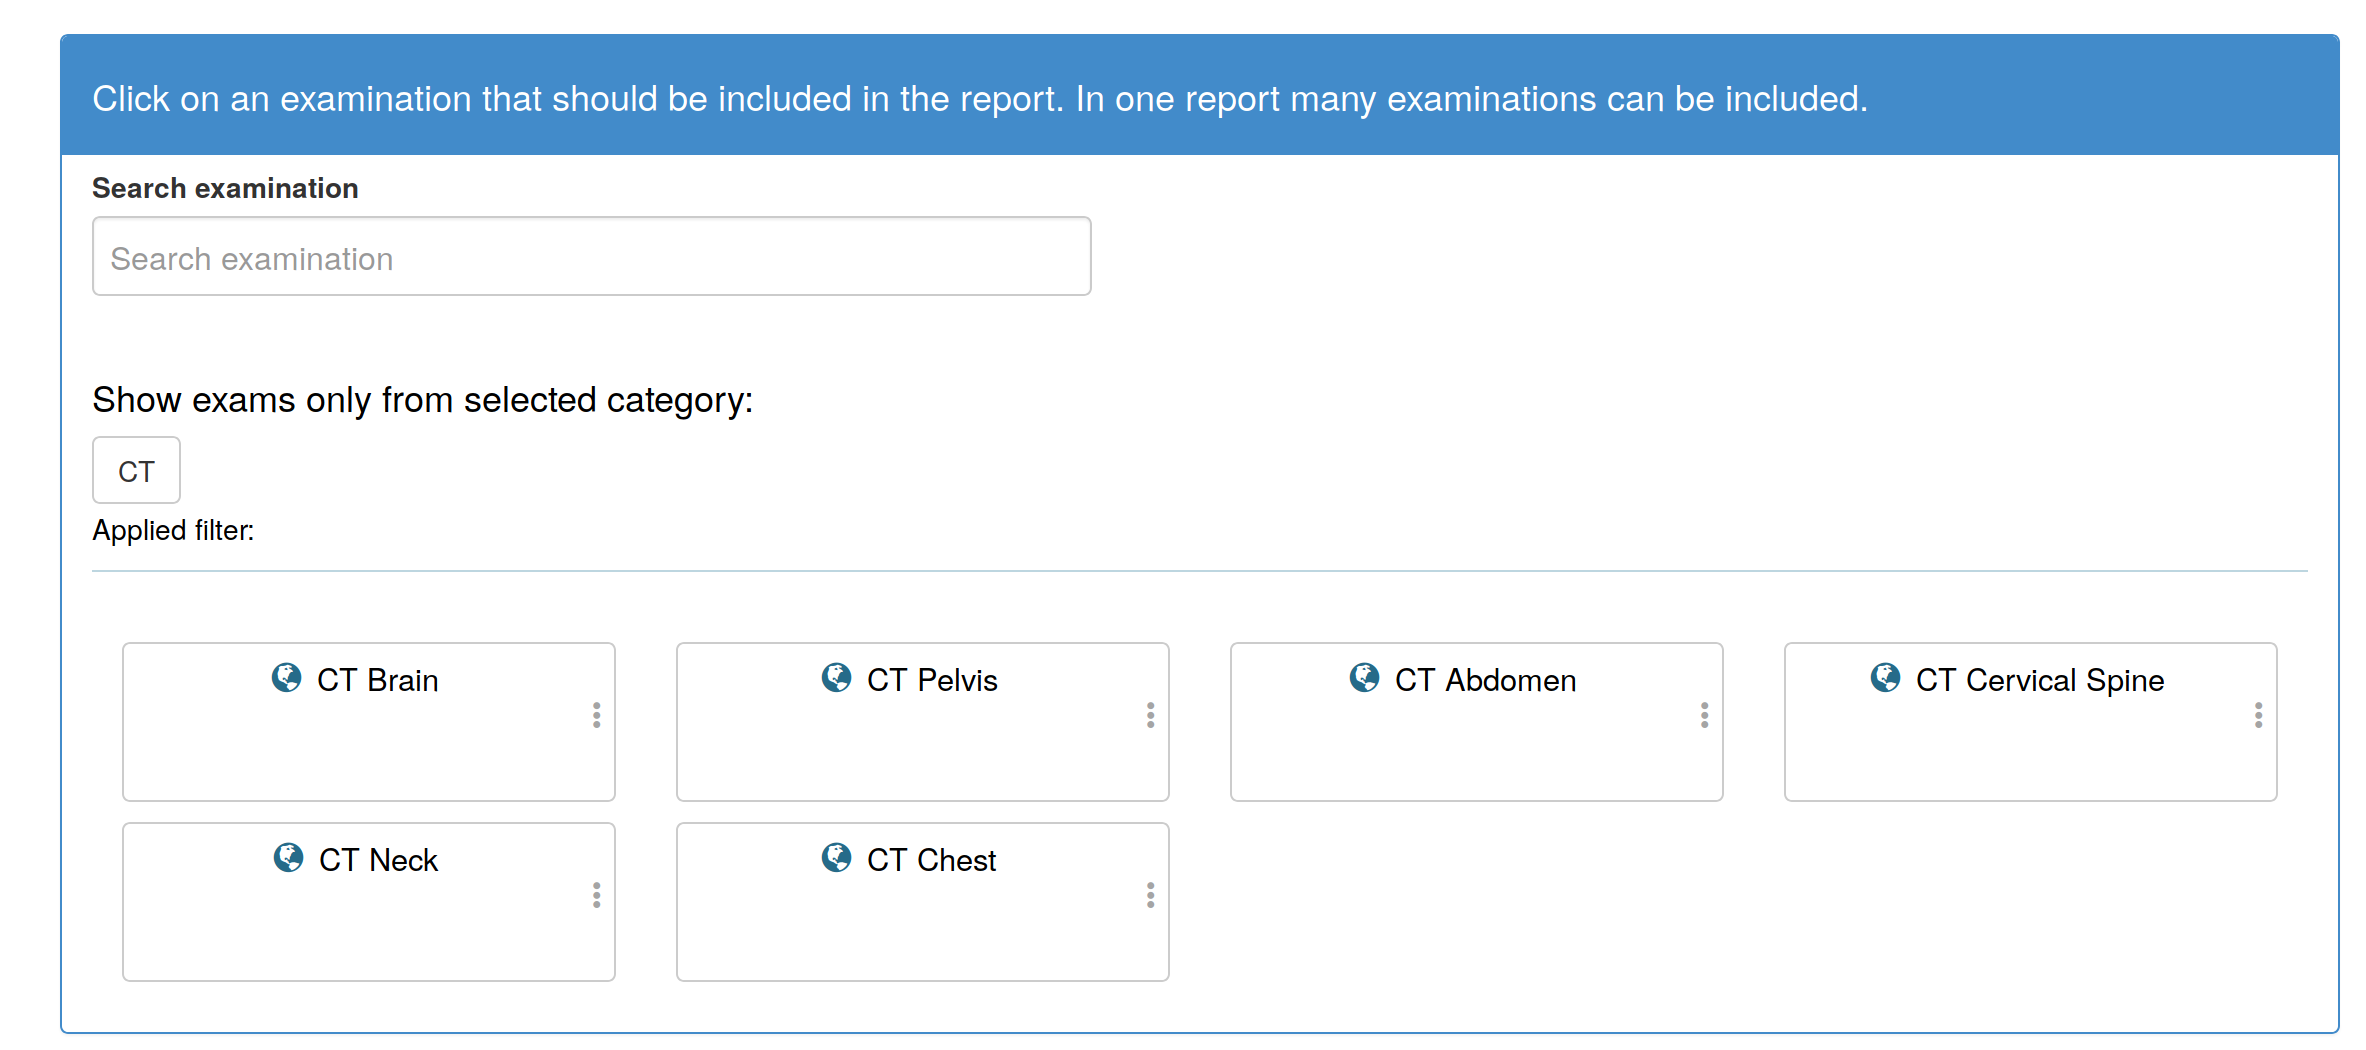
\includegraphics[width=1\linewidth]{../examination-list}
	\label{fig:examination-list}
\end{figure}
\end{frame}

\begin{frame}
\frametitle{Organ list}
\begin{figure}
	\centering
	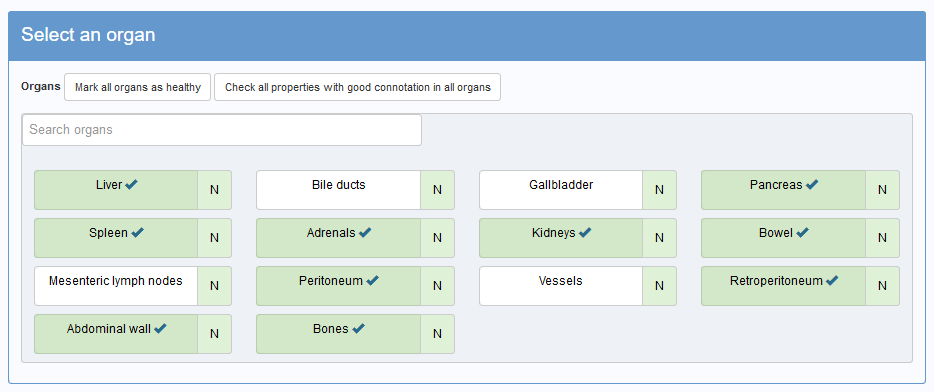
\includegraphics[width=1\linewidth]{../report-organs}
	\label{fig:organ-list}
\end{figure}
\end{frame}

\begin{frame}
\frametitle{Properties}
\begin{figure}
	\centering
	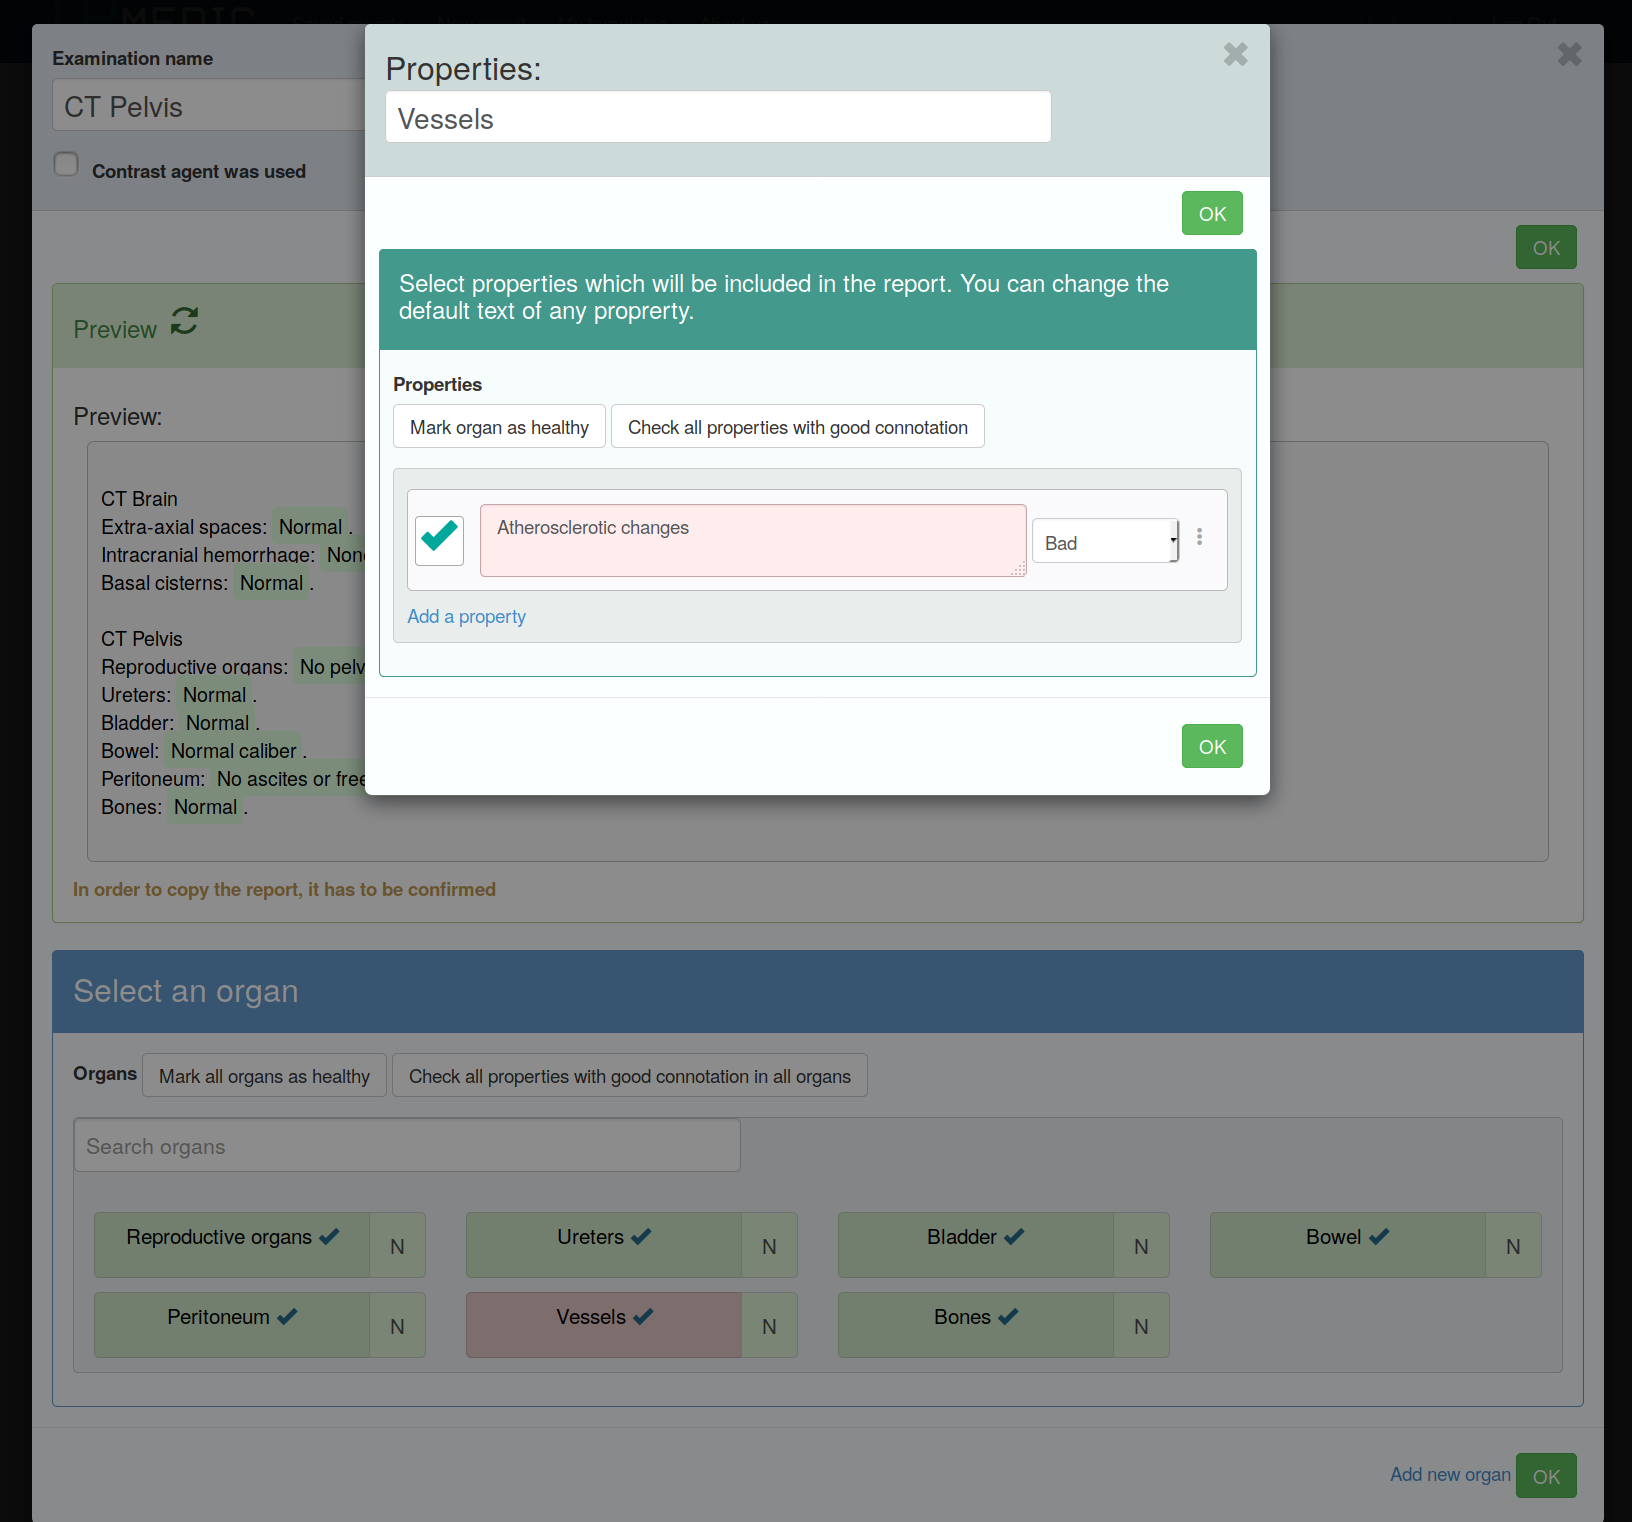
\includegraphics[width=0.8\linewidth]{../properties-modal}
	\label{fig:properties-list}
\end{figure}
\end{frame}

\begin{frame}
\frametitle{Connotations}
\begin{figure}
	\centering
	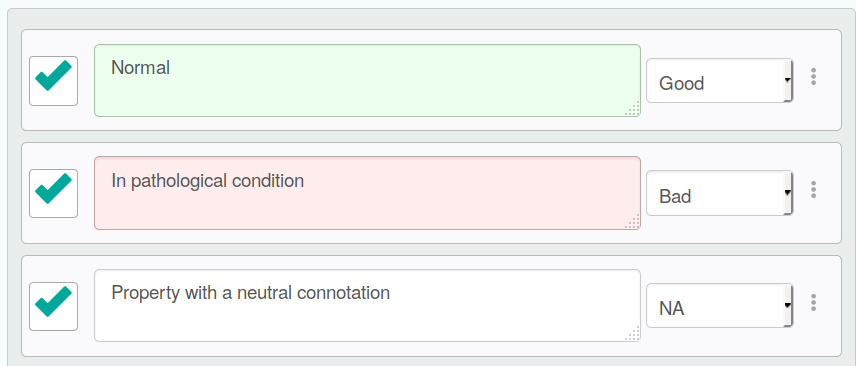
\includegraphics[width=1\linewidth]{../property-connotation}
	\label{fig:property-connotation}
\end{figure}
\end{frame}


\begin{frame}
\frametitle{def. RECIST 1.1}
\begin{figure}
\begin{itemize}
	\item response evaluation criteria in solid tumours
	\item calculates changes in sizes of solid tumors
	\item results based on several factors: change, nodes, selection of measurements
	\end{itemize}
\end{figure}
\end{frame}

\begin{frame}
\frametitle{Parsing values for RECIST 1.1}
\begin{figure}
	\centering
	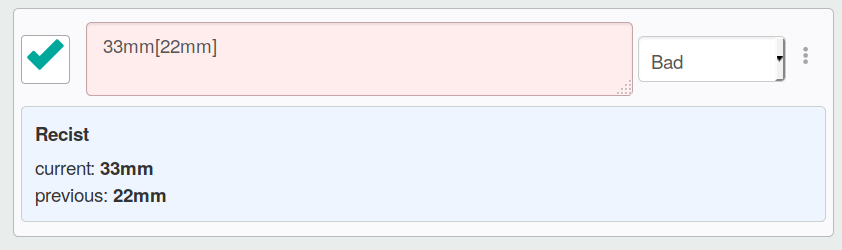
\includegraphics[width=1\linewidth]{../recist-parsing}
	\label{fig:recist-parsing}
\end{figure}
\end{frame}


\begin{frame}
\frametitle{Configuring RECIST 1.1}
\begin{figure}
	\centering
	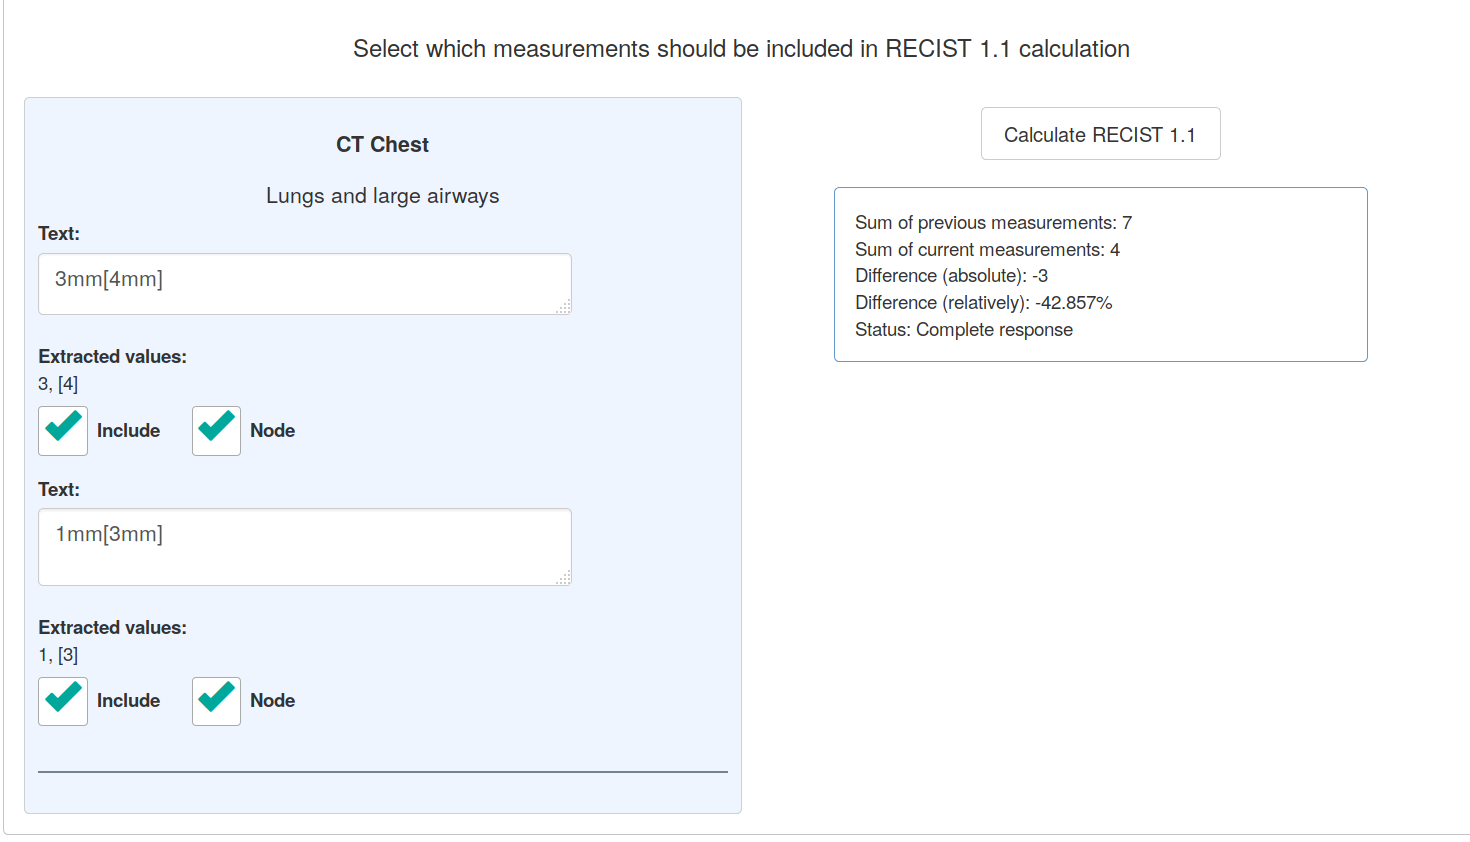
\includegraphics[width=1\linewidth]{../recist-config}
	\label{fig:recist-config}
\end{figure}
\end{frame}


\begin{frame}
\frametitle{Generated report}
\begin{figure}
	\centering
	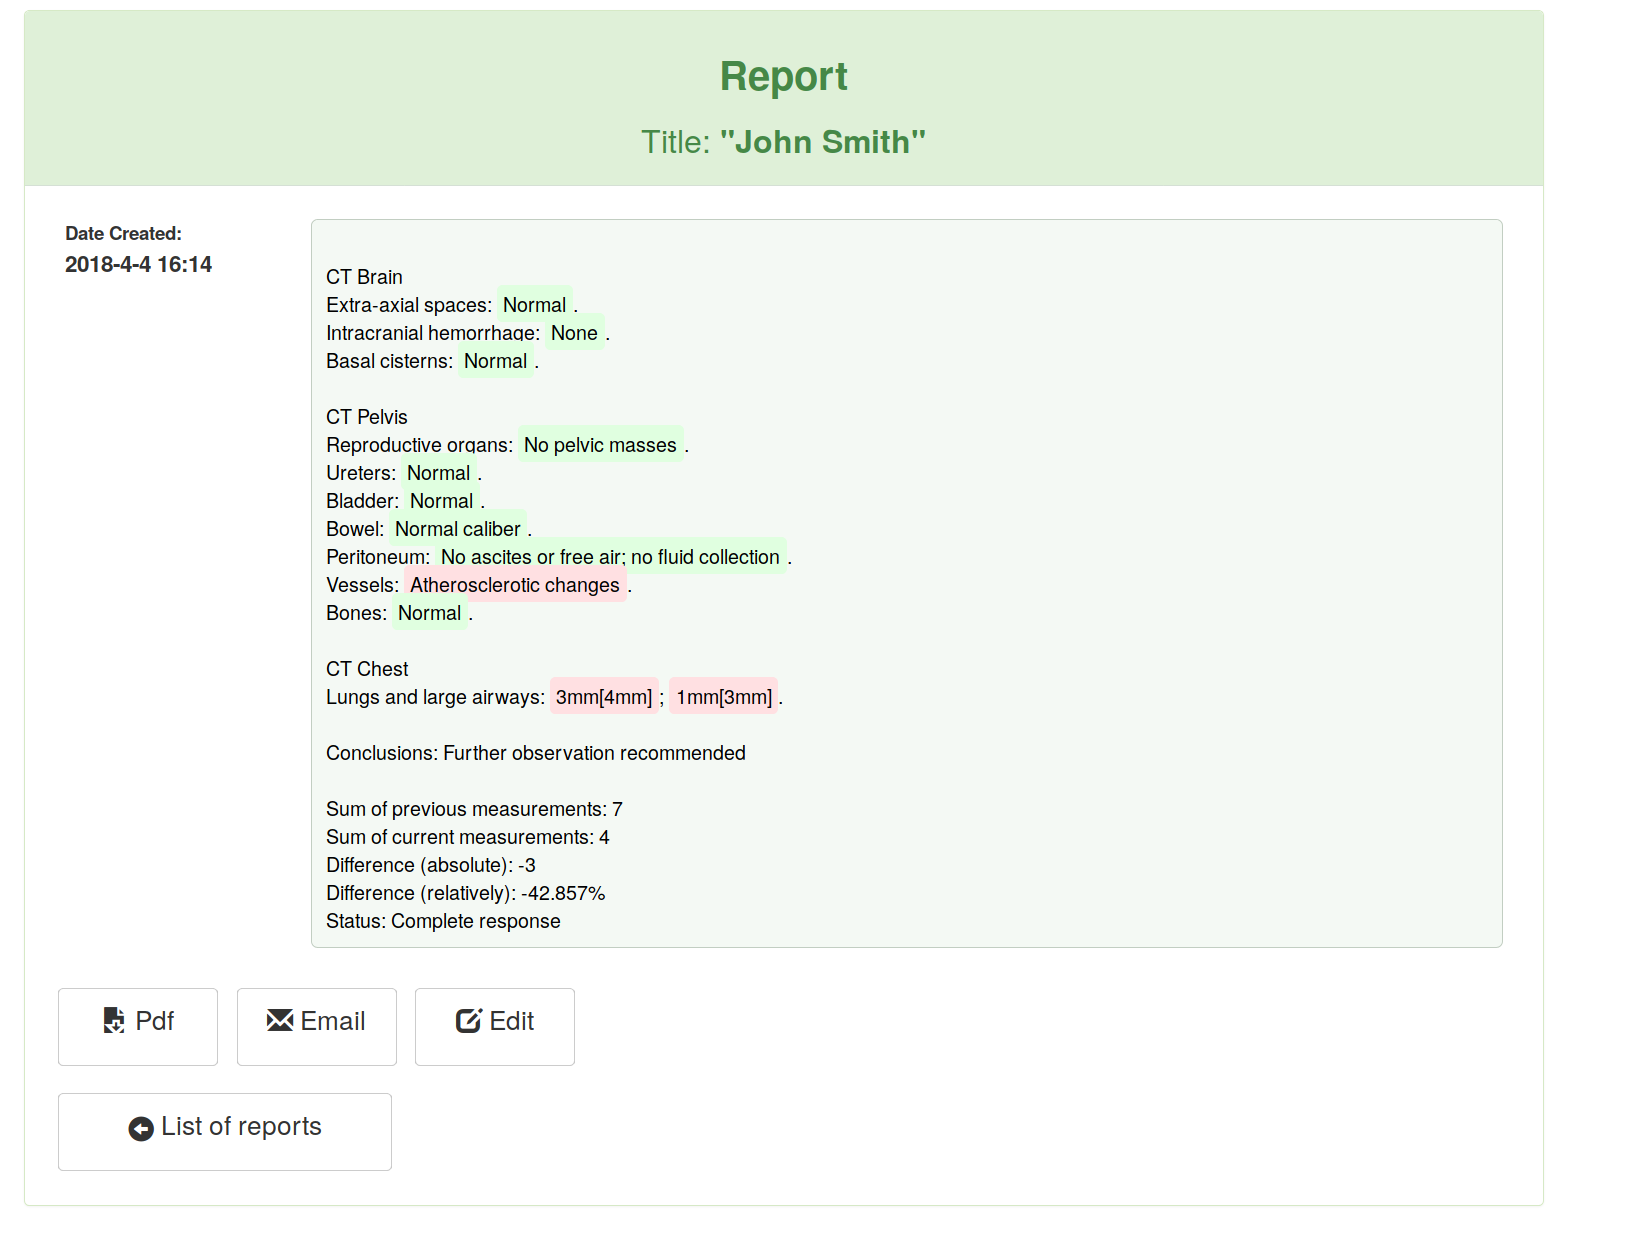
\includegraphics[width=1\linewidth]{../report-copy-to-clipboard}
	\label{fig:report-copy-to-clipboard}
\end{figure}
\end{frame}



\begin{frame}
\frametitle{Template editor}
\begin{figure}
	\centering
	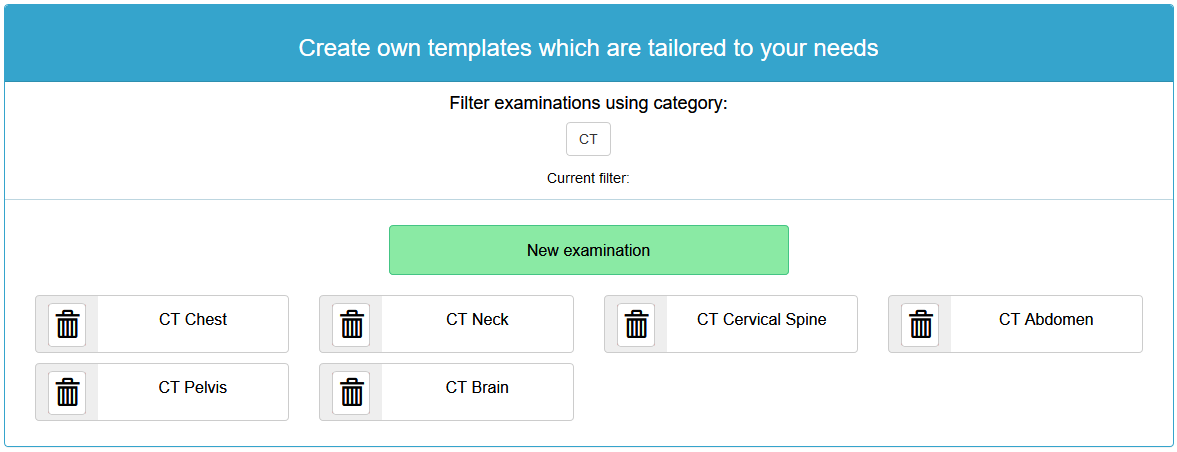
\includegraphics[width=1\linewidth]{../templates-list}
	\label{fig:templates-list}
\end{figure}

\end{frame}
\begin{frame}
\begin{figure}
	\centering
	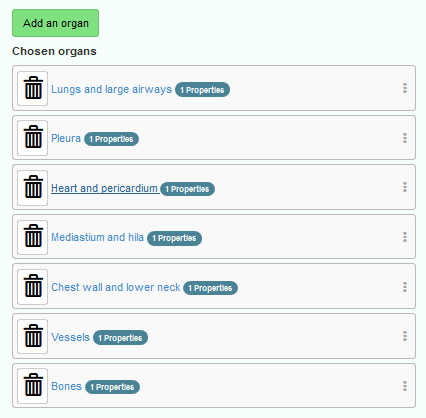
\includegraphics[width=0.5\linewidth]{../template-organs-list}
	\label{fig:template-organ-list}
\end{figure}
\end{frame}

\section {Validation}
\begin{frame}
\frametitle{Validation}
Places where the software was used:
\begin{itemize}
	\item Several independent teleradiologists
	\item Small hospital in Wieliszew
	\item Large network of clinics in Łódź
\end{itemize}

Conclusions:
\begin{itemize}
	\item Tens of thousands reports generated
	\item Reports generated 3 times faster
\end{itemize}
\end{frame}

\section {Plans for the future}
\begin{frame}
\frametitle{Plans for the future}
\begin{itemize}
	\item develop independent commercial version of the software based on some ideas from this system
	\item support for more general ontologies
	\item conform to standards, integrations with existing RIS systems
\end{itemize}
\end{frame}

\begin{frame}
\frametitle{Q\&A}
\end{frame}
\begin{frame}

\frametitle{Bibliography}
\begin{thebibliography}{11}
	\bibitem{bls} https://www.bls.gov/ooh/healthcare/physicians-and-surgeons.htm, accessed 08.10.2017 13:30
	\bibitem{ai} M. Recht, N. Bryan, Artificial Intelligence: Threat or Boon to Radiologists?
	N1  - doi: 10.1016/j.jacr.2017.07.007
	\bibitem{snomed} T. Benson, Principles of health interoperability HL7 and SNOMED.
	\bibitem{sr} D. A. Clunie, DICOM Structured Reporting
	\bibitem{hl7cda} http://www.hl7.org/Special/committees/structure/index.cfm 
	\bibitem{csharp-spec}
	https://docs.microsoft.com/en-us/dotnet/csharp/language-reference/language-specification/lexical-structure
	\bibitem{static-lang}
	S. Hanenberg, S. Kleinschmager, R. Robbes, É. Tanter, A. Stefik, An empirical study on the impact of static typing on software maintainability

\end{thebibliography}
\end{frame}
\end{document}
